\section{Arquitectura de la Solución}

La figura X muestra un diagrama de arquitectura de la solución, para
soportar los procesos de análisis y extracción de datos, así como la
visualización de los mismos.
La participación de cada uno de los componentes de la solución en las distintas
etapas, será explicado en las próximas secciones.

\begin{figure}[H]
  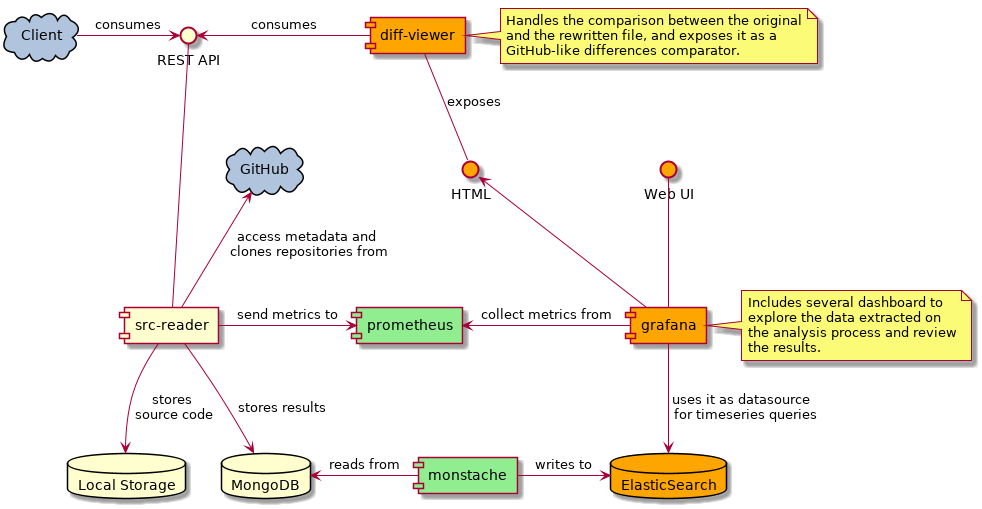
\includegraphics[width=12cm]{implementation/architecture_overview.png}
  \centering
  \caption{Arquitectura general de la Solución}
\end{figure}

\subsection{Fase: Cálculo}

Tal como se enunció anteriormente, la fase de cálculo consta de diferentes etapas,
cada una con un objetivo bien claro.
Estas etapas se suceden unas a otras, utilizando la salida de una estapa previamente
ejecutada, como entrada para la siguiente, presentando así una cierta secuencialidad.

%extracción, procesamiento y cálculo.

\subsubsection{Etapa: Extracción}

Para poder dividir y expandir los identificadores que forman parte de una base de código de fuente, 
primero necesitamos analizar los archivos que lo componen y construir los árboles de sintáxisis
abstracta, que serán procesados en la etapa siguiente.
Los pasos que forman parte 
Este proceso, definido como \textbf{extracción}, y contiene diferentes pasos,
dentro de los que encontramos:

\begin{enumerate}
  \item Clonación de repositorios de código.
  \item Filtrado de archivos.
  \item Construcción de ASTs.
\end{enumerate}

La etapa de extracción inicia con la \textbf{clonación del repositorio} elegido para ser
analizado. En el caso de nuestra solución, se requiere que el código fuente esté
versionado a través de la herramienta de control de versiones (TODO: SVCs, link) de \textit{git},
y disponible públicamente en la plataforma de \textit{GitHub} (TODO: link).
A través de las librerías correspondientes, el código es copiado a un directorio temporal,
para luego ser procesado.

Como no todos los archivos que forman parte de un repositorio son de interés para la construcción
de un árbol de sintáxis abstracta, aquellos que no formen parte del conjunto candidato, son
\textbf{filtrados}.
Esto implica que sólo los archivos de extensión \textit{.go} son considerados, exceptuando
los que tienen el sufijo \textit{\_test.go}, ya que contienen el código para las pruebas
unitarias y/o de integración, y por el momento se decidió descartar.

Por último, con el conjunto de archivos a analizar ya determinado, se procede a la
\textbf{construcción de los árboles de sintáxis abstracta}.
Para ello, el proceso se apoya en las librerías provistas dentro de la distribución
por defecto del lenguaje de programación, las cuales permiten leer los archivos,
hacer la \textit{tokenización} y \textit{parsing} de los mismos, con la consecuente
generación de los ASTs.

%TODO (incluir sección de AST y GO?)
%AST en Golang, convenciones de desarrollo, Effective Go, Levesthein distance.

Como resultado de esta etapa, tenemos un conjunto de ASTs, los cuales sirven como parámetros
de entrada para la etapa de procesamiento, la cual es explicada a continuación.

\subsubsection{Etapa: Procesamiento}

La correcta ejecución de algunos algoritmos, tanto de división como de expansión,
requiere cierta \textbf{información contextual}, extraída desde el código fuente.
Por ejemplo, y tal como se especificó en el capítulo X, el algorimo de división \textit{Samurai}
depende de dos tablas de frencuencias.
Una de estas tablas es específica al programa bajo análisis, mientras que la otra corresponde
a un universo mayor de código fuente, independiente del código en cuestión.
Así mismo, el algoritmo de \textit{Expansión Básica} utiliza listas tanto de palabras como frases,
extraídas de los comentarios e identificadores asociados a cada una de las funciones analizadas.
En el caso de \textit{AMAP}, para poder efectuar las expansiones, se necesitan establecer tablas
de frecuencia por métodos, clases, paquetes e incluso proyectos.

Esta información contextual necesaria, se extrae durante la etapa de \textbf{procesamiento},
al realizar un \textbf{análisis semántico} sobre los diferentes \textit{árboles de sintáxis abstracta (ASTs)} 
resultantes del paso anterior.

\subsubsection{Etapa: Cálculo}

Durante la etapa de \textbf{cálculo}, los identificadores son relevados desde el código fuente,
y los distintos algoritmos aplicados.
La aplicación de los algoritmos se hace de a pares, con una combinación preestablecida
entre división y expansión.

La expansión resultante, junto con el nombre original del identificador, son las
entradas para el cálculo de la métrica, aplicando la distancia de Levesthein
entre ambos.
De esta manera, se obtiene un valor que representa la distancia entre los mismos.

Cada identificador, junto con sus separaciones y expansiones obtenidas por los diferentes
algoritmos, y el valor de la métrica, son almacenadas en una base de datos.
De esta manera, luego es posible combinar los valores de cada, agregándolos al nivel
que se desee explorar (paquete o proyecto).

\subsection{Fase: Visualización}

Una vez completada la fase de cálculo, los resultados quedan disponibles para la
visualización de los mismos.
Para ello, hay dos componentes particulares.
Por un lado, el componente que permite la visualización de las métricas por proyecto,
a nivel general; y por otro, la herramienta que permite previsualizar un archivo
de código fuente, cambiando los nombres de los identificadores por su mejor expansión,
de acuerdo al valor de la métrica.

Las siguientes secciones explican al detalle los elementos de visualización, y
la forma correcta de interpretarlos.

\subsubsection{Visualización: Dashboards}

Para analizar la información extraída desde cada uno de los proyectos, el componente
principal de visualización se apoya en un conjunto de tableros construidos sobre
\textit{Grafana} (TODO, insertar link).
Tal como se comentó en la \textbf{fase de procesamiento}, los resultados de cada proyecto
son almacenados en una base de datos, y luego replicados a una instancia de \textit{ElasticSearch}.
De esta manera, a través de los tableros se puede acceder a la información obtenida,
además de poder trabajar sobre ella, principalmente en operaciones de agrupamientos
y búsquedas.

Accesibles desde la instancia de Grafana, existen varios dashboards, cada uno con
un propósito específico.

Los detalles de cada uno de los dashboards, son provistos a continuación.

\paragraph{Insights Overview}
El dashboard encargado de sumarizar las métricas de evaluación de distancia de las
expansiones con su nombre original, a nivel de proyecto y su exploración por paquetes,
es el tablero de \textit{Insights}.

\begin{figure}[H]
  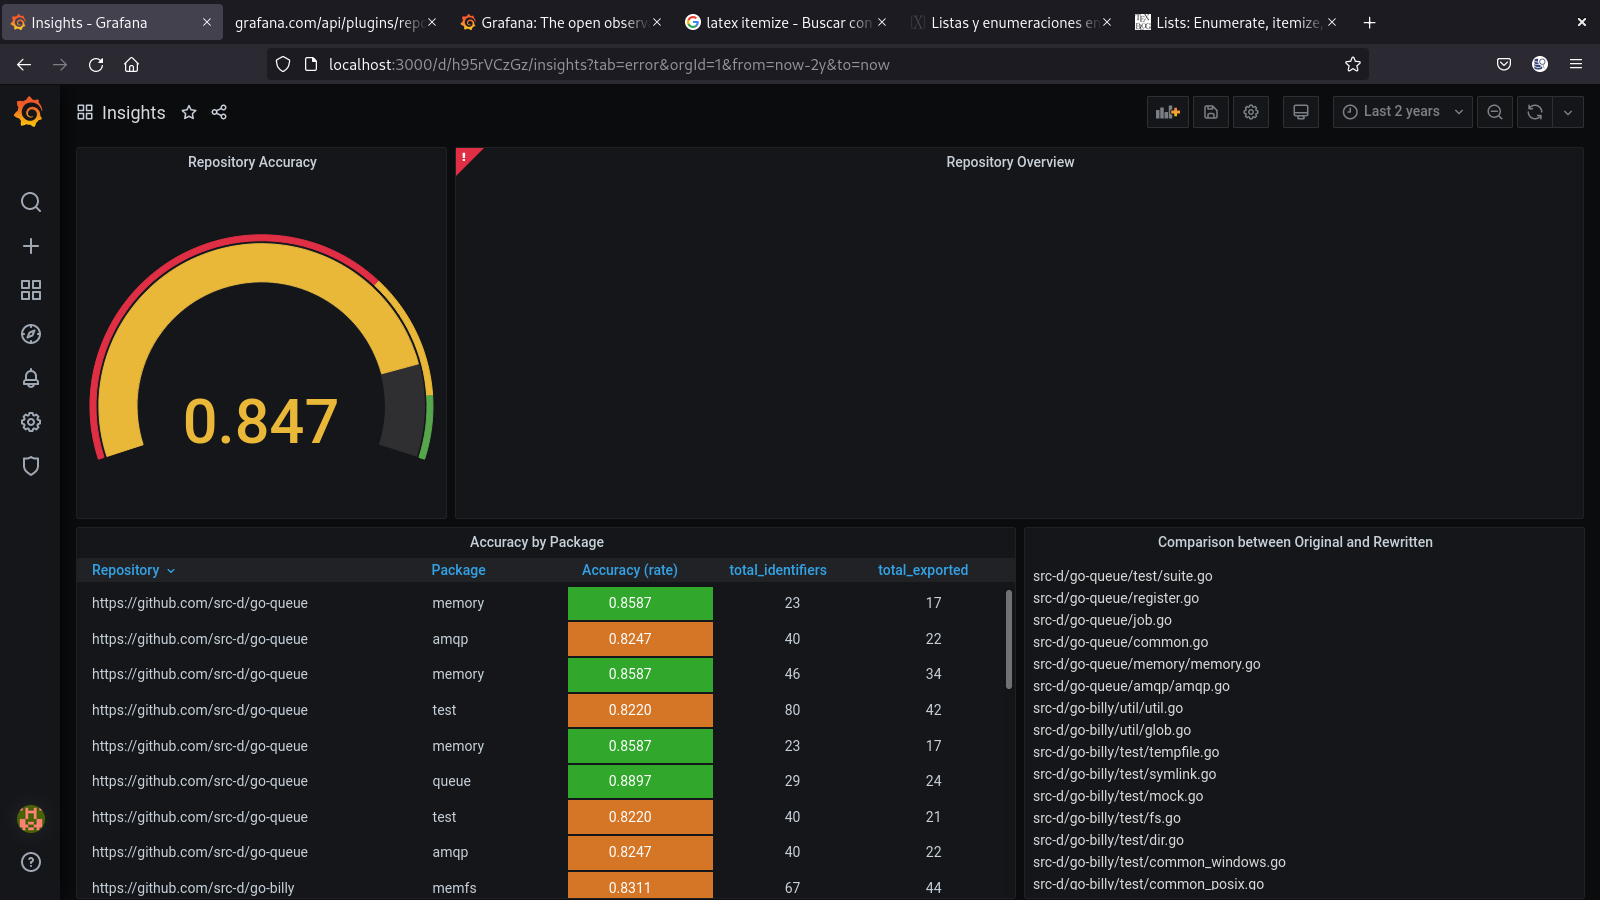
\includegraphics[width=12cm]{implementation/dashboard_insights_overview.png}
  \centering
  \caption{Dashboard: Insights Overview}
\end{figure}

Como demuestra la figura X, este tablero permite visualizar:

\begin{itemize}
  \item Efectividad del nombramiento, a través de la métrica de distancia aplicada
  a los identificadores.
  \item Efectividad del proyecto, paquete por paquete, incluyendo la cantidad de identificadores
  en los mismos, y su impacto dada su condición de exportado o no.
\end{itemize}

Además, permite el acceso a la visualización de \textbf{Rewrite}, partiendo desde la lista de archivos
que componen al proyecto en cuestión.
Esta visualización es descrita luego, en su sección correspondiente.

Este tablero es quizás el más importante, ya que nos permite \textbf{evaluar la calidad del proyecto},
comparando los resultados agregados de la métrica, contra unos rangos de valores esperados
previamente definidos.
Para este informe, los rangos de aceptación fueron establecidos empíricamente (TODO: ?),
y se encuentra en el orden de:

\textit{TODO: agregar tabla de valores esperados.}

\paragraph{Analysis Overview}
Este dashboard (\textit{Analysis Overview}, dado su nombre en inglés en la herramienta)
permite observar los proyectos desde la perspectiva de post-ejecución de la fase
de cálculo, y más puntualmente de las etapas que incluyen la división y expansión
de los indicadores.
Una pre-visualización del mismo se puede ver en la figura X, donde aparecen las
principales métricas que el dashboard expone.
Dentro de este conjunto podemos encontrar:

\begin{itemize}
  \item Cantidad de análisis realizados, junto con los pre-procesadores aplicados y las
  combinaciones de algoritmos divisores y expansores.
  \item Número total de archivos procesados, separando entre aquellos que no tuvieron
  problemas de los que sí presentaron errores durante la ejecución.
  \item Número total de indicadores extraídos, separando entre aquellos que no tuvieron
  problemas de los que sí presentaron errores durante su procesamiento.
  \item Lista de proyectos analizados hasta el momento, con sus detalles sobre archivos
  procesados e indicadores extraídos, siempre considerando los que fueron válidos y los
  que presentaron algún inconveniente.
\end{itemize}

\begin{figure}[H]
  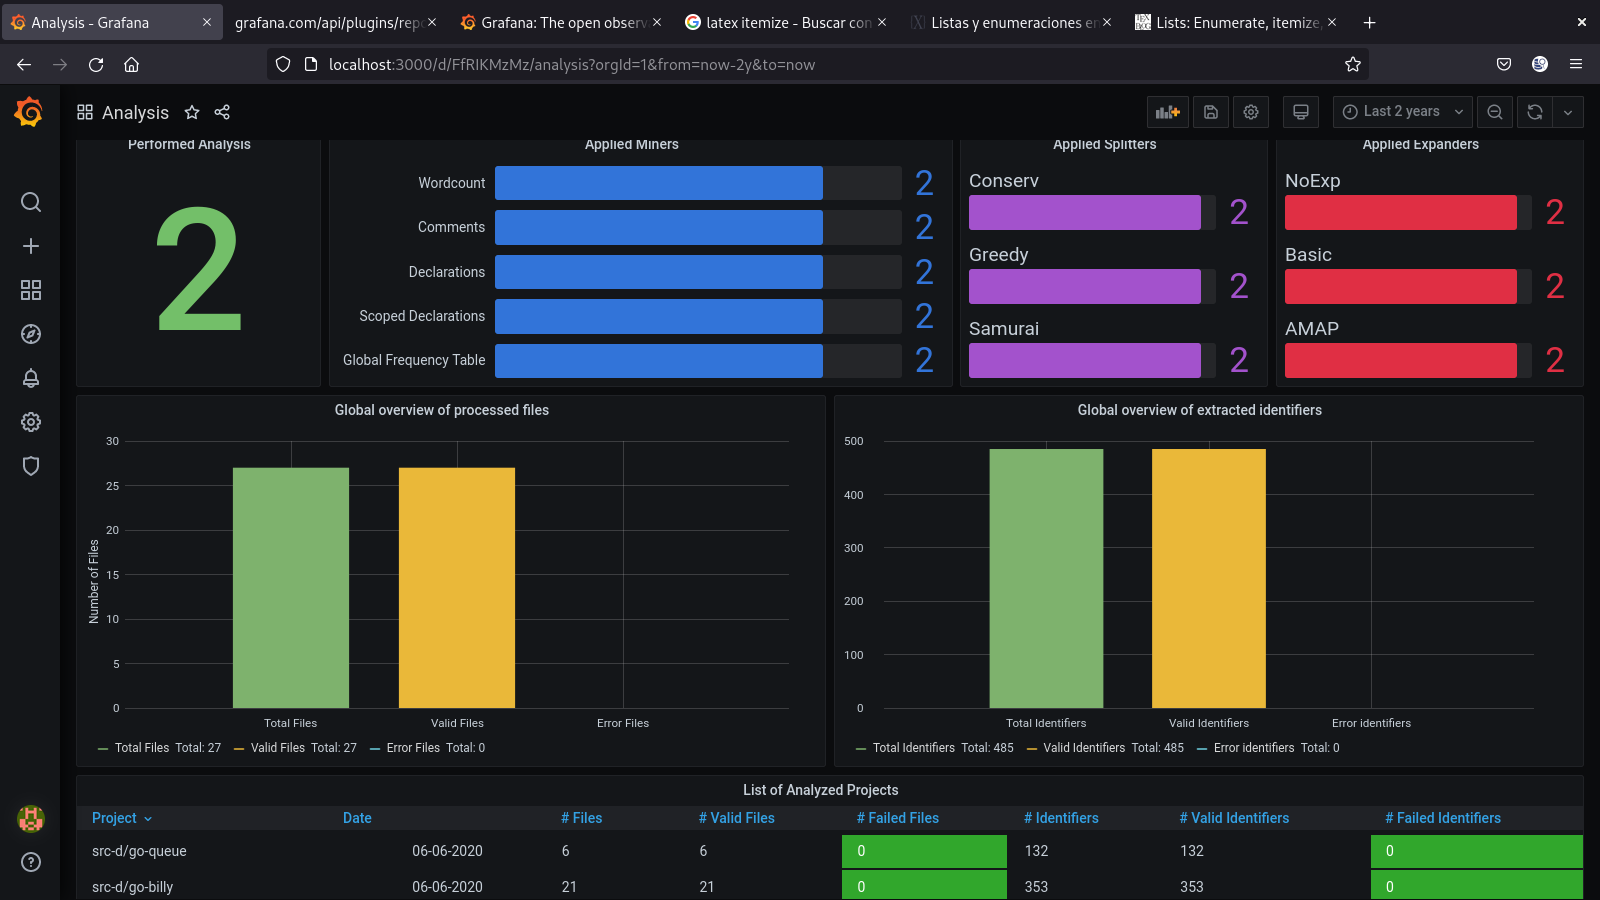
\includegraphics[width=12cm]{implementation/dashboard_analysis_overview.png}
  \centering
  \caption{Dashboard: Analysis Overview}
\end{figure}

\paragraph{Identifiers Overview}
En este tablero (\textit{Identifiers Overview}, dado su nombre en inglés en la herramienta)
ayuda a hacer un análisis respecto a los indicadores procesados, a nivel global, pero
dejando de lado las particularidades de cada proyecto.
De esta manera, podemos acceder a las siguientes métricas globales sobre los tipos de
identificadores que se están procesando:

\begin{itemize}
  \item Cantidad de identificadores extraídos a nivel global, y promedio por proyecto.
  \item Distribución por tipo (\textit{var, struct, interface, func, const}) de los
  identificadores procesados (tanto en cantidad como porcentaje).
  \item Identificadores a nivel de paquete, exportados o no (tanto en cantidad como porcentaje).
\end{itemize}

\begin{figure}[H]
  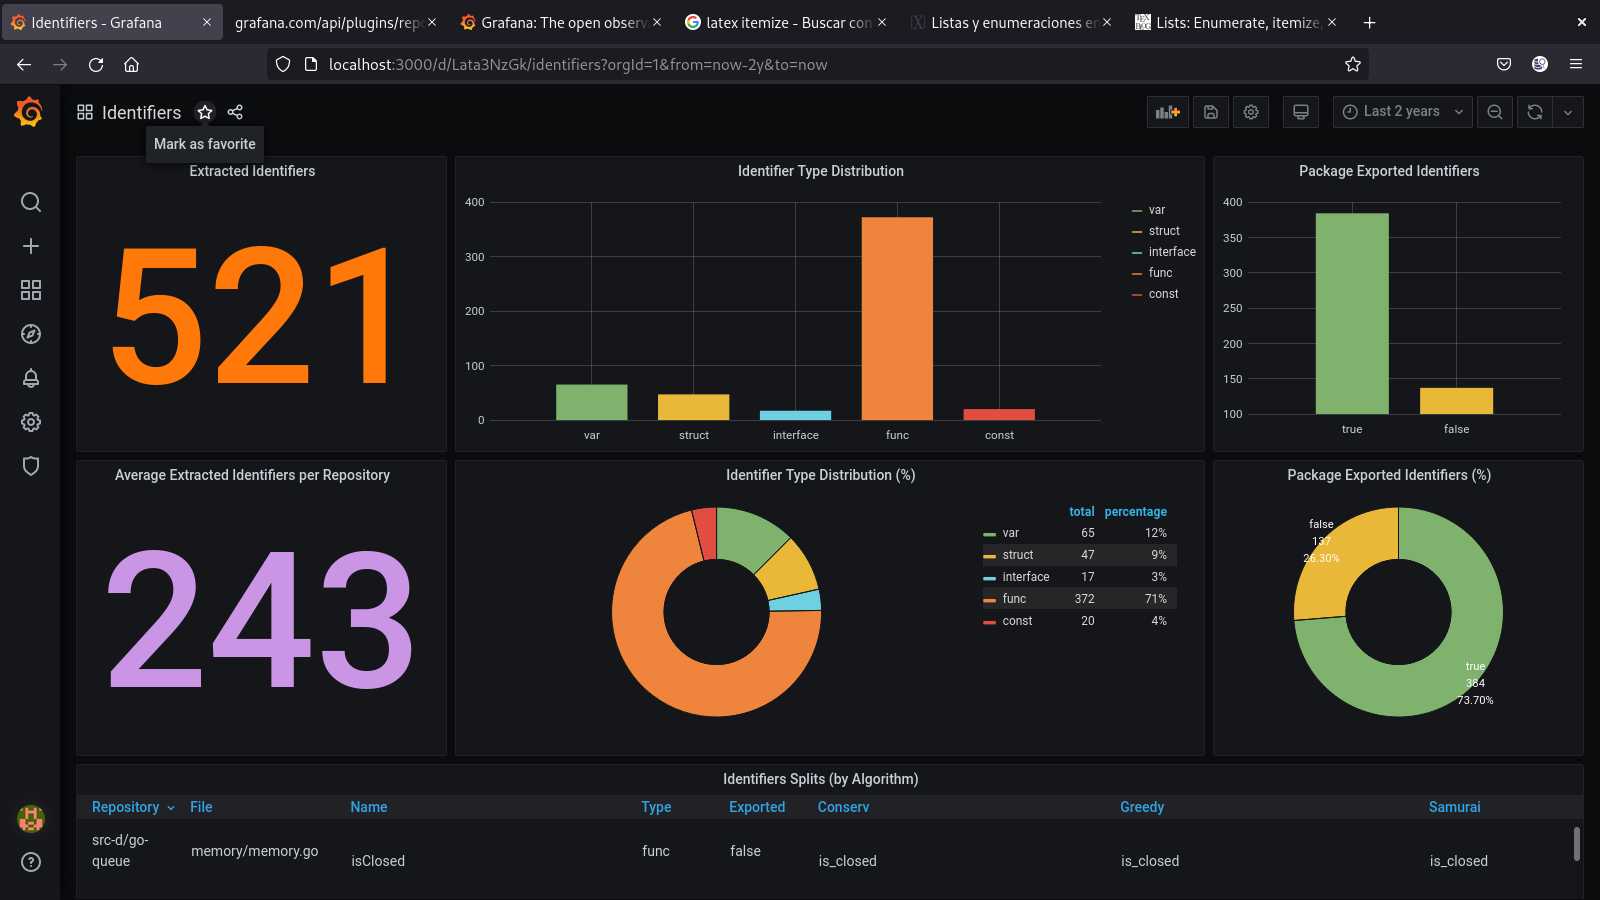
\includegraphics[width=12cm]{implementation/dashboard_identifiers_details_part1.png}
  \centering
  \caption{Dashboard: Identifiers Overview - Métricas generales}
\end{figure}

Así mismo, tal como muestra la figura X, también se pueden visualizar los resultados
de la aplicación de los diferentes algoritmos de división y expansión, por cada uno
de los identificadores evaluados.
Para ello, se utilizan unas tablas que indican detalles básicamos del identificador,
como el proyecto al que pertenece, el archivo en que se encuentra, su nombre, su tipo,
si es exportado o no.
Junto con esta información básica, se muestran los resultados de los algoritmos de división
por un lado, y por otro, los de los algoritmos de expansión (incluyendo varias opciones en
caso que el algoritmo las arroje).

\begin{figure}[H]
  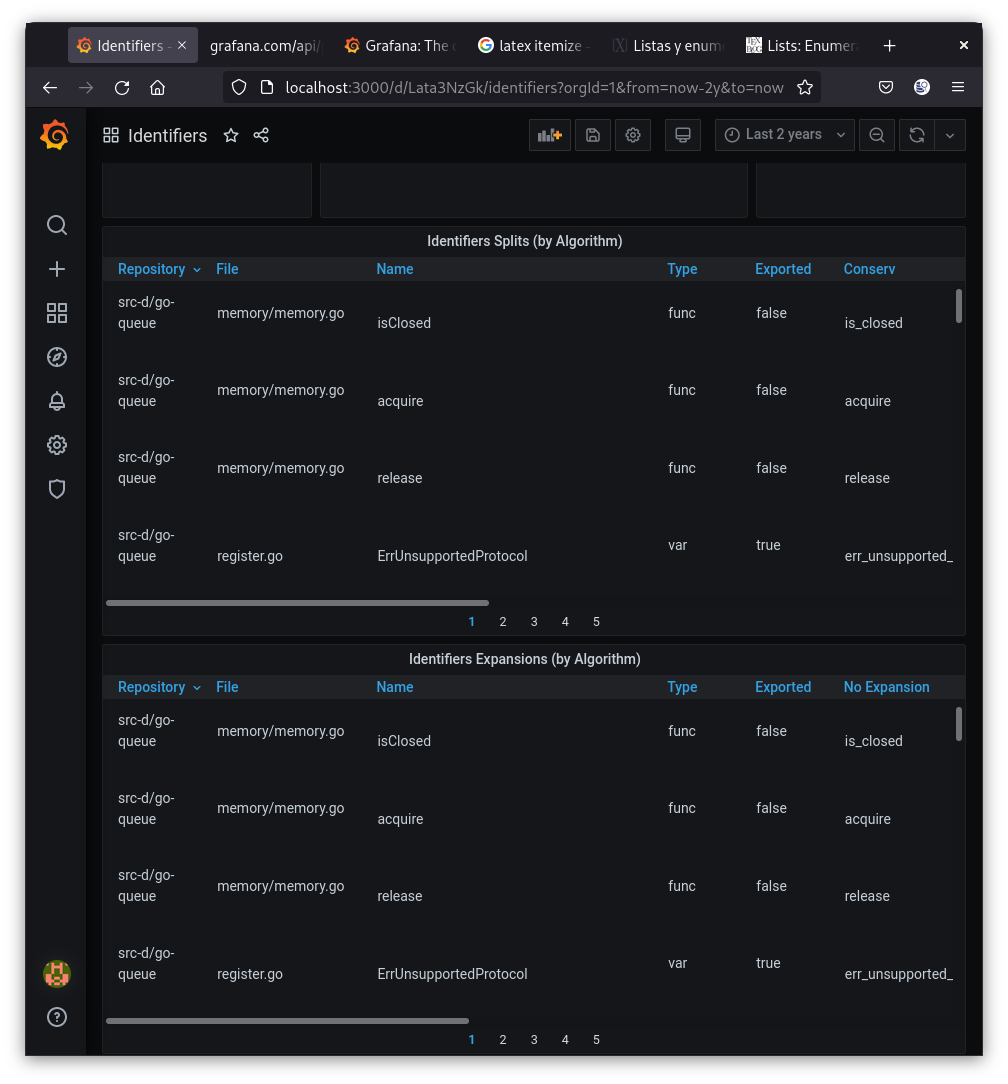
\includegraphics[width=12cm]{implementation/dashboard_identifiers_details_part2.png}
  \centering
  \caption{Dashboard: Identifiers Overview - Divisiones y expansiones}
\end{figure}

\paragraph{Projects Overview}
Por último, el tablero de visualización de Proyectos (\textit{Projects Overview}),
nos brinda \textbf{información contextual} sobre los repositorios analizados,
como puede apreciarse en la figura X.
Estos datos nos permiten conocer particularidades de los proyectos, ya que
podemos observar la cantidad de repositorios considerados, en qué momento fueron creados y
las licencias que aplican.
Además, también se puede conocer la cantidad promedio de archivos que los componen y su
tamaño promedio (en bytes).

De esta manera, podemos entender mejor ciertas características sobre los proyectos que pueden
impactar sobre la evaluación de la métrica de distancia en los distintos identificadores.

\begin{figure}[H]
  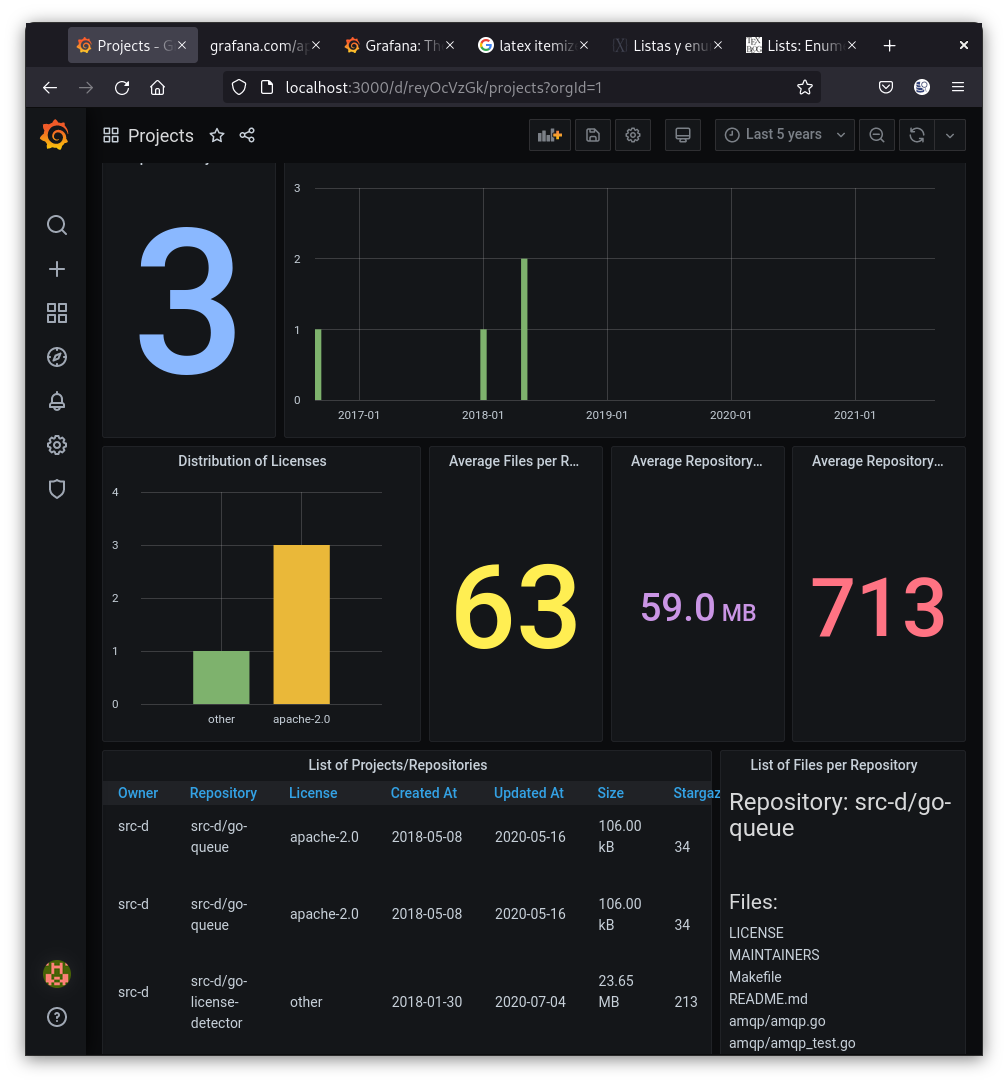
\includegraphics[width=12cm]{implementation/dashboard_projects_overview.png}
  \centering
  \caption{Dashboard: Projects Overview}
\end{figure}

\subsubsection{Visualización: Rewrite}

La previsualización del reemplazo de los identificadores de un archivo
por el resultado del procesamiento de división, expansión y cálculo de distancia,
se realiza por medio de la herramienta \textsc{diff-viewer}.

Esta herramienta presenta una disposición similar al comparador de código
disponible en GitHub, donde se resalta tanto la línea de código como el texto modificado,
tal como puede verse en la figura X.

\begin{figure}[H]
  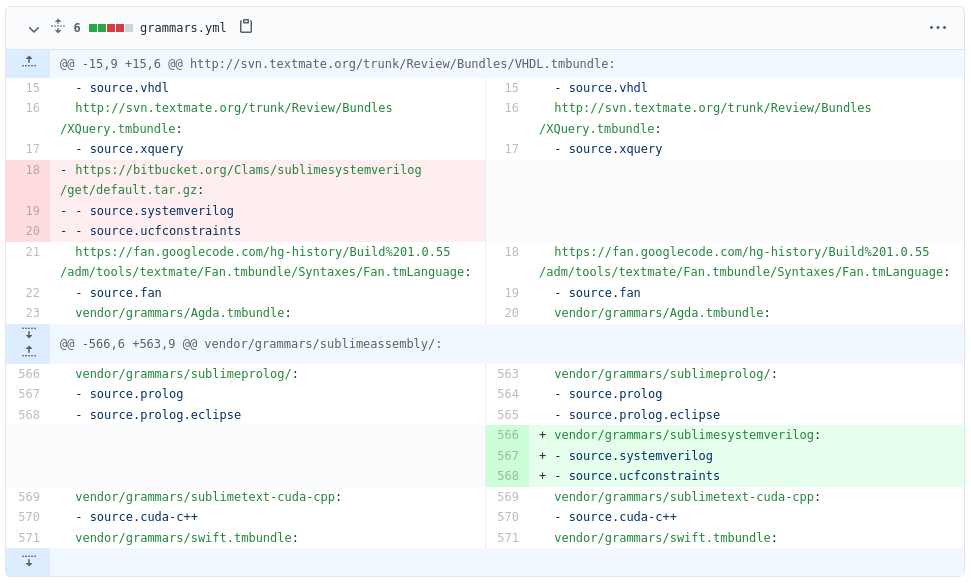
\includegraphics[width=12cm]{implementation/github_comparator.png}
  \centering
  \caption{Comparador de cambios de GitHub}
\end{figure}

Dentro del conjunto de información brindada por la herramienta, se destacan
dos elementos particulares.

Por un lado, el usuario final puede hacerse una idea general de qué tan acorde
o no es el nombramiento de los identificadores en un archivo particular, al
visualizar la \textbf{cantidad total de modificaciones} entre la versión original
y la sobreescrita.
Como la previsualización de reescritura sólo se enfoca en cambiar nombres de
indicadores, el valor de sustracciones y adiciones siempre va a ser el mismo, con
signo cambiado.
Por ello, es el valor absoluto de cualquiera de las dos mediciones, el que nos
determina la magnitud de indicadores con potenciales mejoras.

Así mismo, la herramienta nos permite \textbf{previsualizar línea por línea}, cuál sería
el fragmento modificado, y cómo quedaría con el nuevo nombre de indentificador,
extraído del proceso de evaluación.
Tal como puede observarse en la figura X, la línea donde se impacta el cambio
es marcada con un verde claro, mientras que el nombre del identificador sugerido
(y siendo éste el cambio efectivo) se representa con un verde más oscuro, para
poder destacarse.

\begin{figure}[H]
  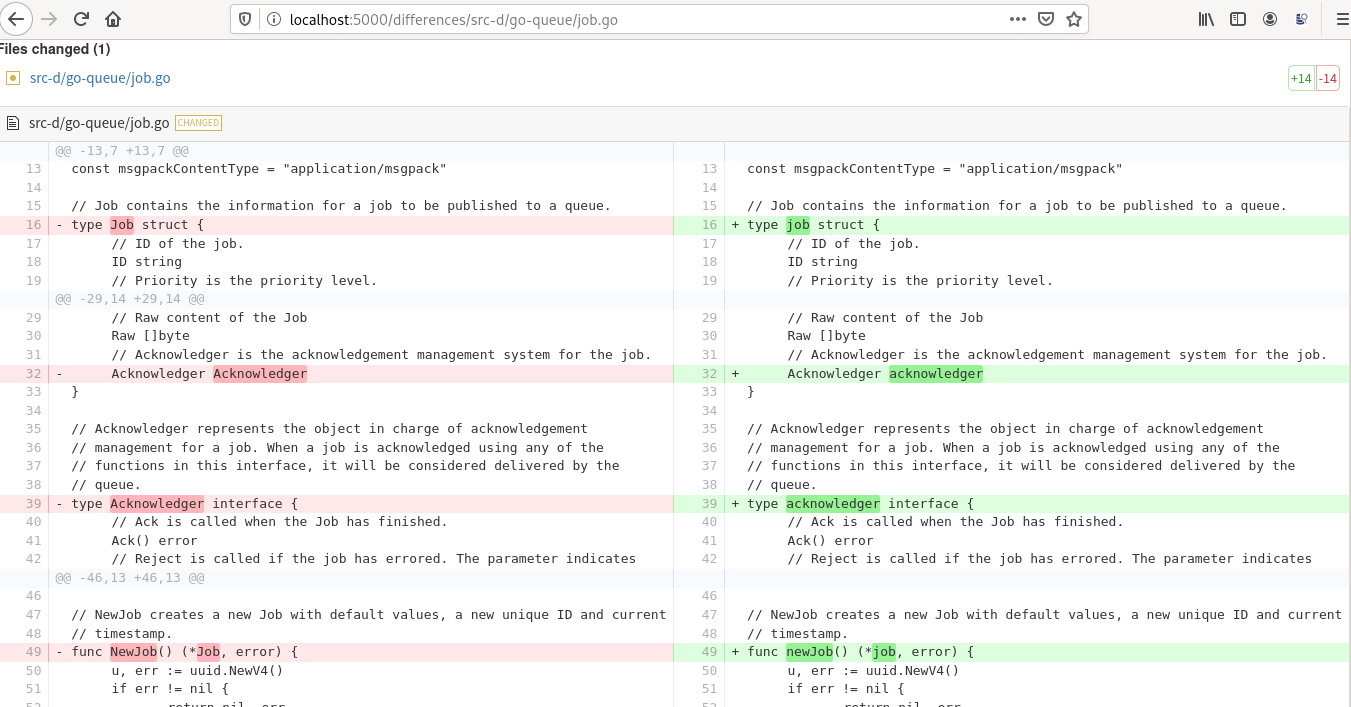
\includegraphics[width=12cm]{implementation/diff_viewer.png}
  \centering
  \caption{Previsualización de Diferencias}
\end{figure}

\textit{TODO: agregar cajas para marcar los dos puntos anteriores en la imagen.}
